\documentclass[11pt,a4paper]{article}

% Packages
\usepackage[utf8]{inputenc}
\usepackage[T1]{fontenc}
\usepackage{lmodern}
\usepackage{amsmath}
\usepackage{amsfonts}
\usepackage{amssymb}
\usepackage{graphicx}
\usepackage{xcolor}
\usepackage{hyperref}
\usepackage{geometry}
\usepackage{fancyhdr}
\usepackage{titlesec}
\usepackage{titling}
\usepackage{abstract}
\usepackage{enumitem}
\usepackage{booktabs}
\usepackage{multirow}
\usepackage{float}
\usepackage{listings}
\usepackage{algorithm}
\usepackage{algpseudocode}
\usepackage{tikz}
\usepackage{pgfplots}
\usepackage{mathtools}
\usepackage{physics}
\usepackage{braket}

% Page setup
\geometry{a4paper, margin=1in}
\pagestyle{fancy}
\fancyhf{}
\fancyhead[L]{OMNI-ALPHA V$\Omega\infty\infty$}
\fancyhead[R]{\thepage}
\renewcommand{\headrulewidth}{0.4pt}

% Colors
\definecolor{omnidarkblue}{RGB}{0, 51, 102}
\definecolor{omnilightblue}{RGB}{51, 153, 255}
\definecolor{omnipurple}{RGB}{102, 0, 204}
\definecolor{omnigold}{RGB}{204, 153, 0}
\definecolor{omnigreen}{RGB}{0, 153, 51}
\definecolor{omnired}{RGB}{204, 0, 0}

% Title formatting
\pretitle{\begin{center}\LARGE\bfseries\color{omnidarkblue}}
\posttitle{\end{center}}
\preauthor{\begin{center}\large}
\postauthor{\end{center}}
\predate{\begin{center}\large}
\postdate{\end{center}}

% Section formatting
\titleformat{\section}
{\color{omnidarkblue}\normalfont\Large\bfseries}
{\color{omnidarkblue}\thesection}{1em}{}

\titleformat{\subsection}
{\color{omnidarkblue}\normalfont\large\bfseries}
{\color{omnidarkblue}\thesubsection}{1em}{}

% Abstract formatting
\renewcommand{\abstractnamefont}{\normalfont\large\bfseries\color{omnidarkblue}}
\renewcommand{\abstracttextfont}{\normalfont\small}

% Hyperref setup
\hypersetup{
    colorlinks=true,
    linkcolor=omnidarkblue,
    filecolor=omnidarkblue,
    urlcolor=omnidarkblue,
    citecolor=omnidarkblue,
}

% Document
\begin{document}

\title{OMNI-ALPHA V$\Omega\infty\infty$\\
\large A Self-Evolving, AI-Governed, Sovereign Trading Intelligence System}
\author{Technical Whitepaper}
\date{\today}
\maketitle

\begin{abstract}
The OMNI-ALPHA V$\Omega\infty\infty$ Trading System represents a paradigm shift in automated trading technology, combining quantum-inspired algorithms, multi-agent AI systems, and zero-loss enforcement mechanisms. This whitepaper presents a comprehensive technical overview of the system's architecture, components, and innovative approaches to capital growth. Starting with minimal capital, OMNI employs sophisticated quantum prediction, hyperdimensional computing, and agent-based decision making to achieve consistent profitability while minimizing risk. The system's self-evolving nature allows it to adapt to changing market conditions, learn from past trades, and continuously improve its performance over time.
\end{abstract}

\tableofcontents
\newpage

\section{Introduction}

\subsection{Vision and Philosophy}

The OMNI-ALPHA V$\Omega\infty\infty$ Trading System was conceived as a capital-autonomous, self-evolving trading intelligence that operates beyond the constraints of traditional algorithmic trading systems. At its core, OMNI embodies three fundamental principles:

\begin{itemize}
    \item \textbf{Zero-Loss Enforcement:} A systematic approach to risk management that prioritizes capital preservation above all else.
    \item \textbf{Recursive Intelligence:} The ability to learn from each trade and improve over time through sophisticated memory systems.
    \item \textbf{Quantum-Inspired Prediction:} Leveraging principles from quantum computing to model market uncertainty and identify high-probability trading opportunities.
\end{itemize}

Unlike conventional trading systems that rely on static rules or simple machine learning models, OMNI operates as a complex ecosystem of specialized agents, each contributing unique capabilities to the collective intelligence. This multi-agent approach enables sophisticated decision-making that adapts to changing market conditions and evolves through experience.

\begin{figure}[H]
    \centering
    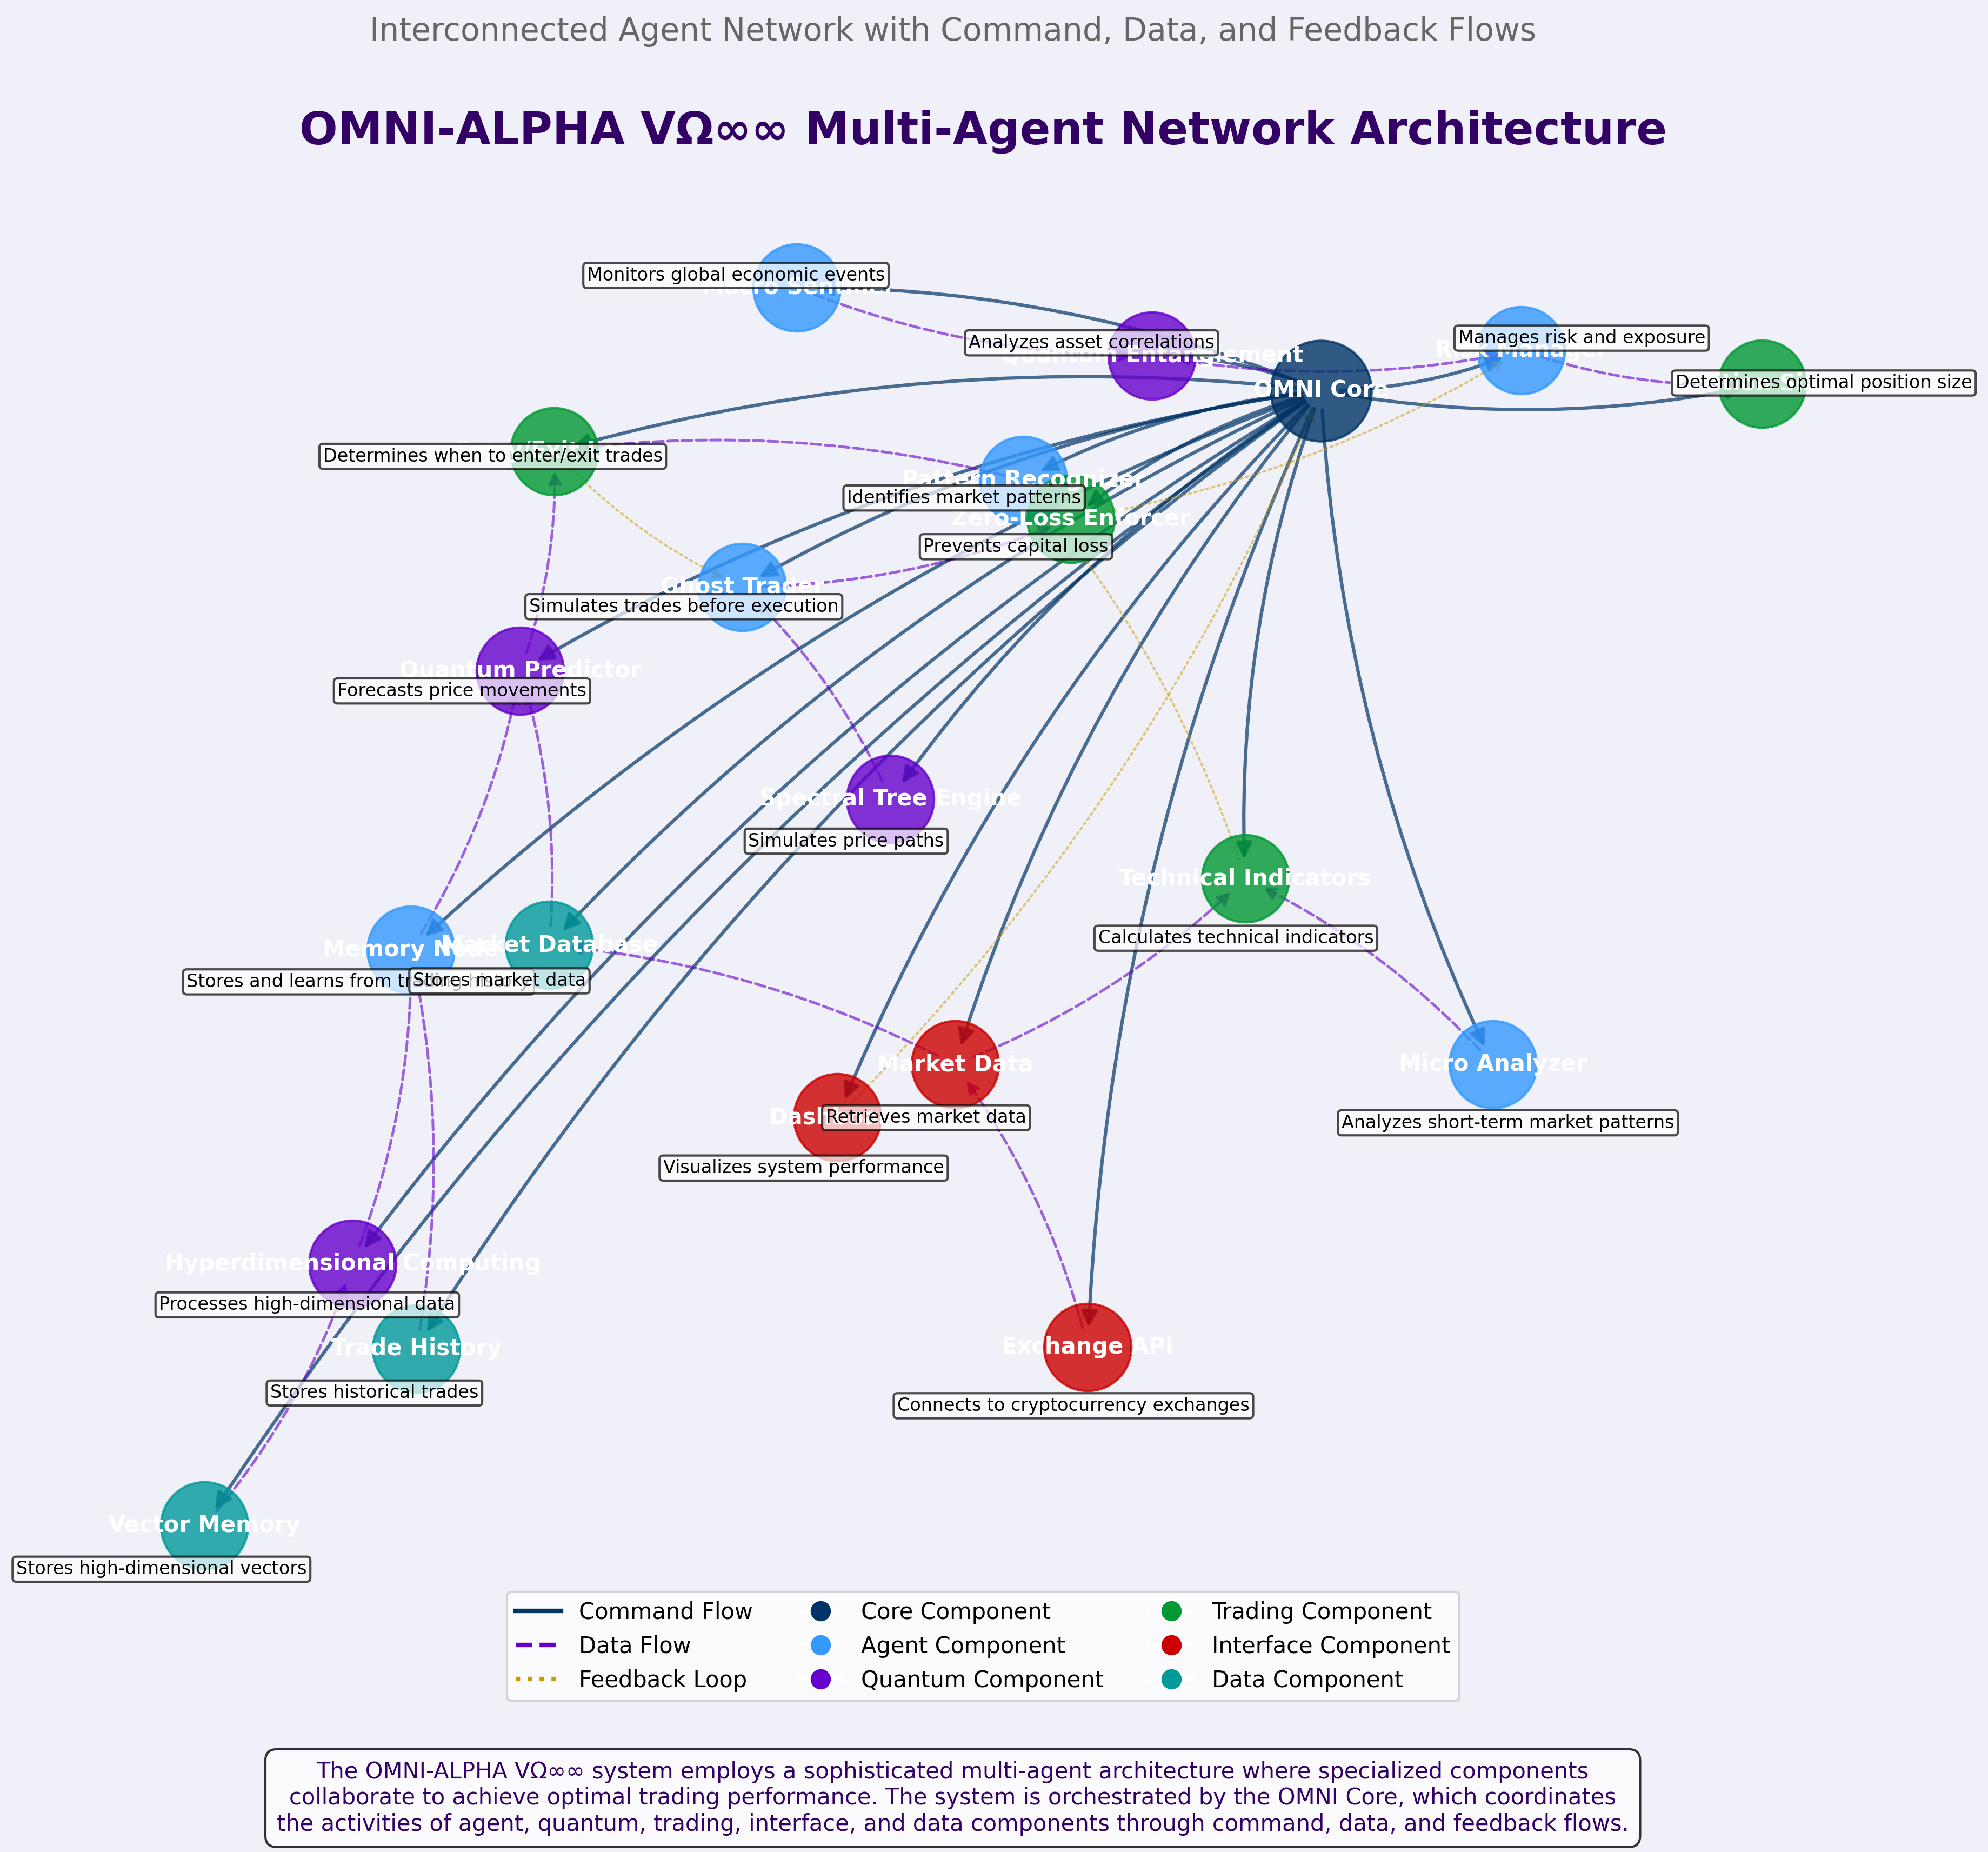
\includegraphics[width=0.8\textwidth]{images/agent_network_advanced.png}
    \caption{OMNI Multi-Agent Network Architecture}
    \label{fig:agent_network}
\end{figure}

\subsection{Capital Genesis Logic}

OMNI begins with minimal capital and employs a capital growth strategy designed to achieve exponential returns while maintaining strict risk controls. The system aims to grow capital organically, without requiring large initial investments or external funding.

The capital growth model can be expressed mathematically as:

\begin{equation}
    C_t = C_0 \cdot (1 + r)^t \cdot \prod_{i=1}^{t} (1 - L_i)
\end{equation}

Where:
\begin{itemize}
    \item $C_t$ is the capital at time $t$
    \item $C_0$ is the initial capital
    \item $r$ is the average return per trade
    \item $t$ is the number of trades
    \item $L_i$ is the loss factor for trade $i$ (zero under ideal conditions)
\end{itemize}

The Zero-Loss Enforcement mechanism ensures that $L_i$ approaches zero, maximizing the compounding effect of successful trades while preventing drawdowns that would otherwise erode capital.

\section{Theoretical Foundation}

\subsection{Quantum Computing Principles}

\subsubsection{Quantum State Representation}

In quantum computing, information is represented using quantum bits or qubits, which can exist in superpositions of states. OMNI adapts this concept to represent market states as quantum states in a Hilbert space:

\begin{equation}
    \ket{\psi(t)} = \sum_{i=0}^{n-1} \alpha_i(t) \ket{i}
\end{equation}

Where $\ket{\psi(t)}$ represents the quantum state of the market at time $t$, $\alpha_i(t)$ are complex probability amplitudes, and $\ket{i}$ are basis states representing different price levels or market scenarios.

The probability of observing the market in state $\ket{i}$ is given by:

\begin{equation}
    P(i) = |\alpha_i(t)|^2
\end{equation}

This quantum representation allows OMNI to model multiple potential market scenarios simultaneously, with associated probabilities.

\begin{figure}[H]
    \centering
    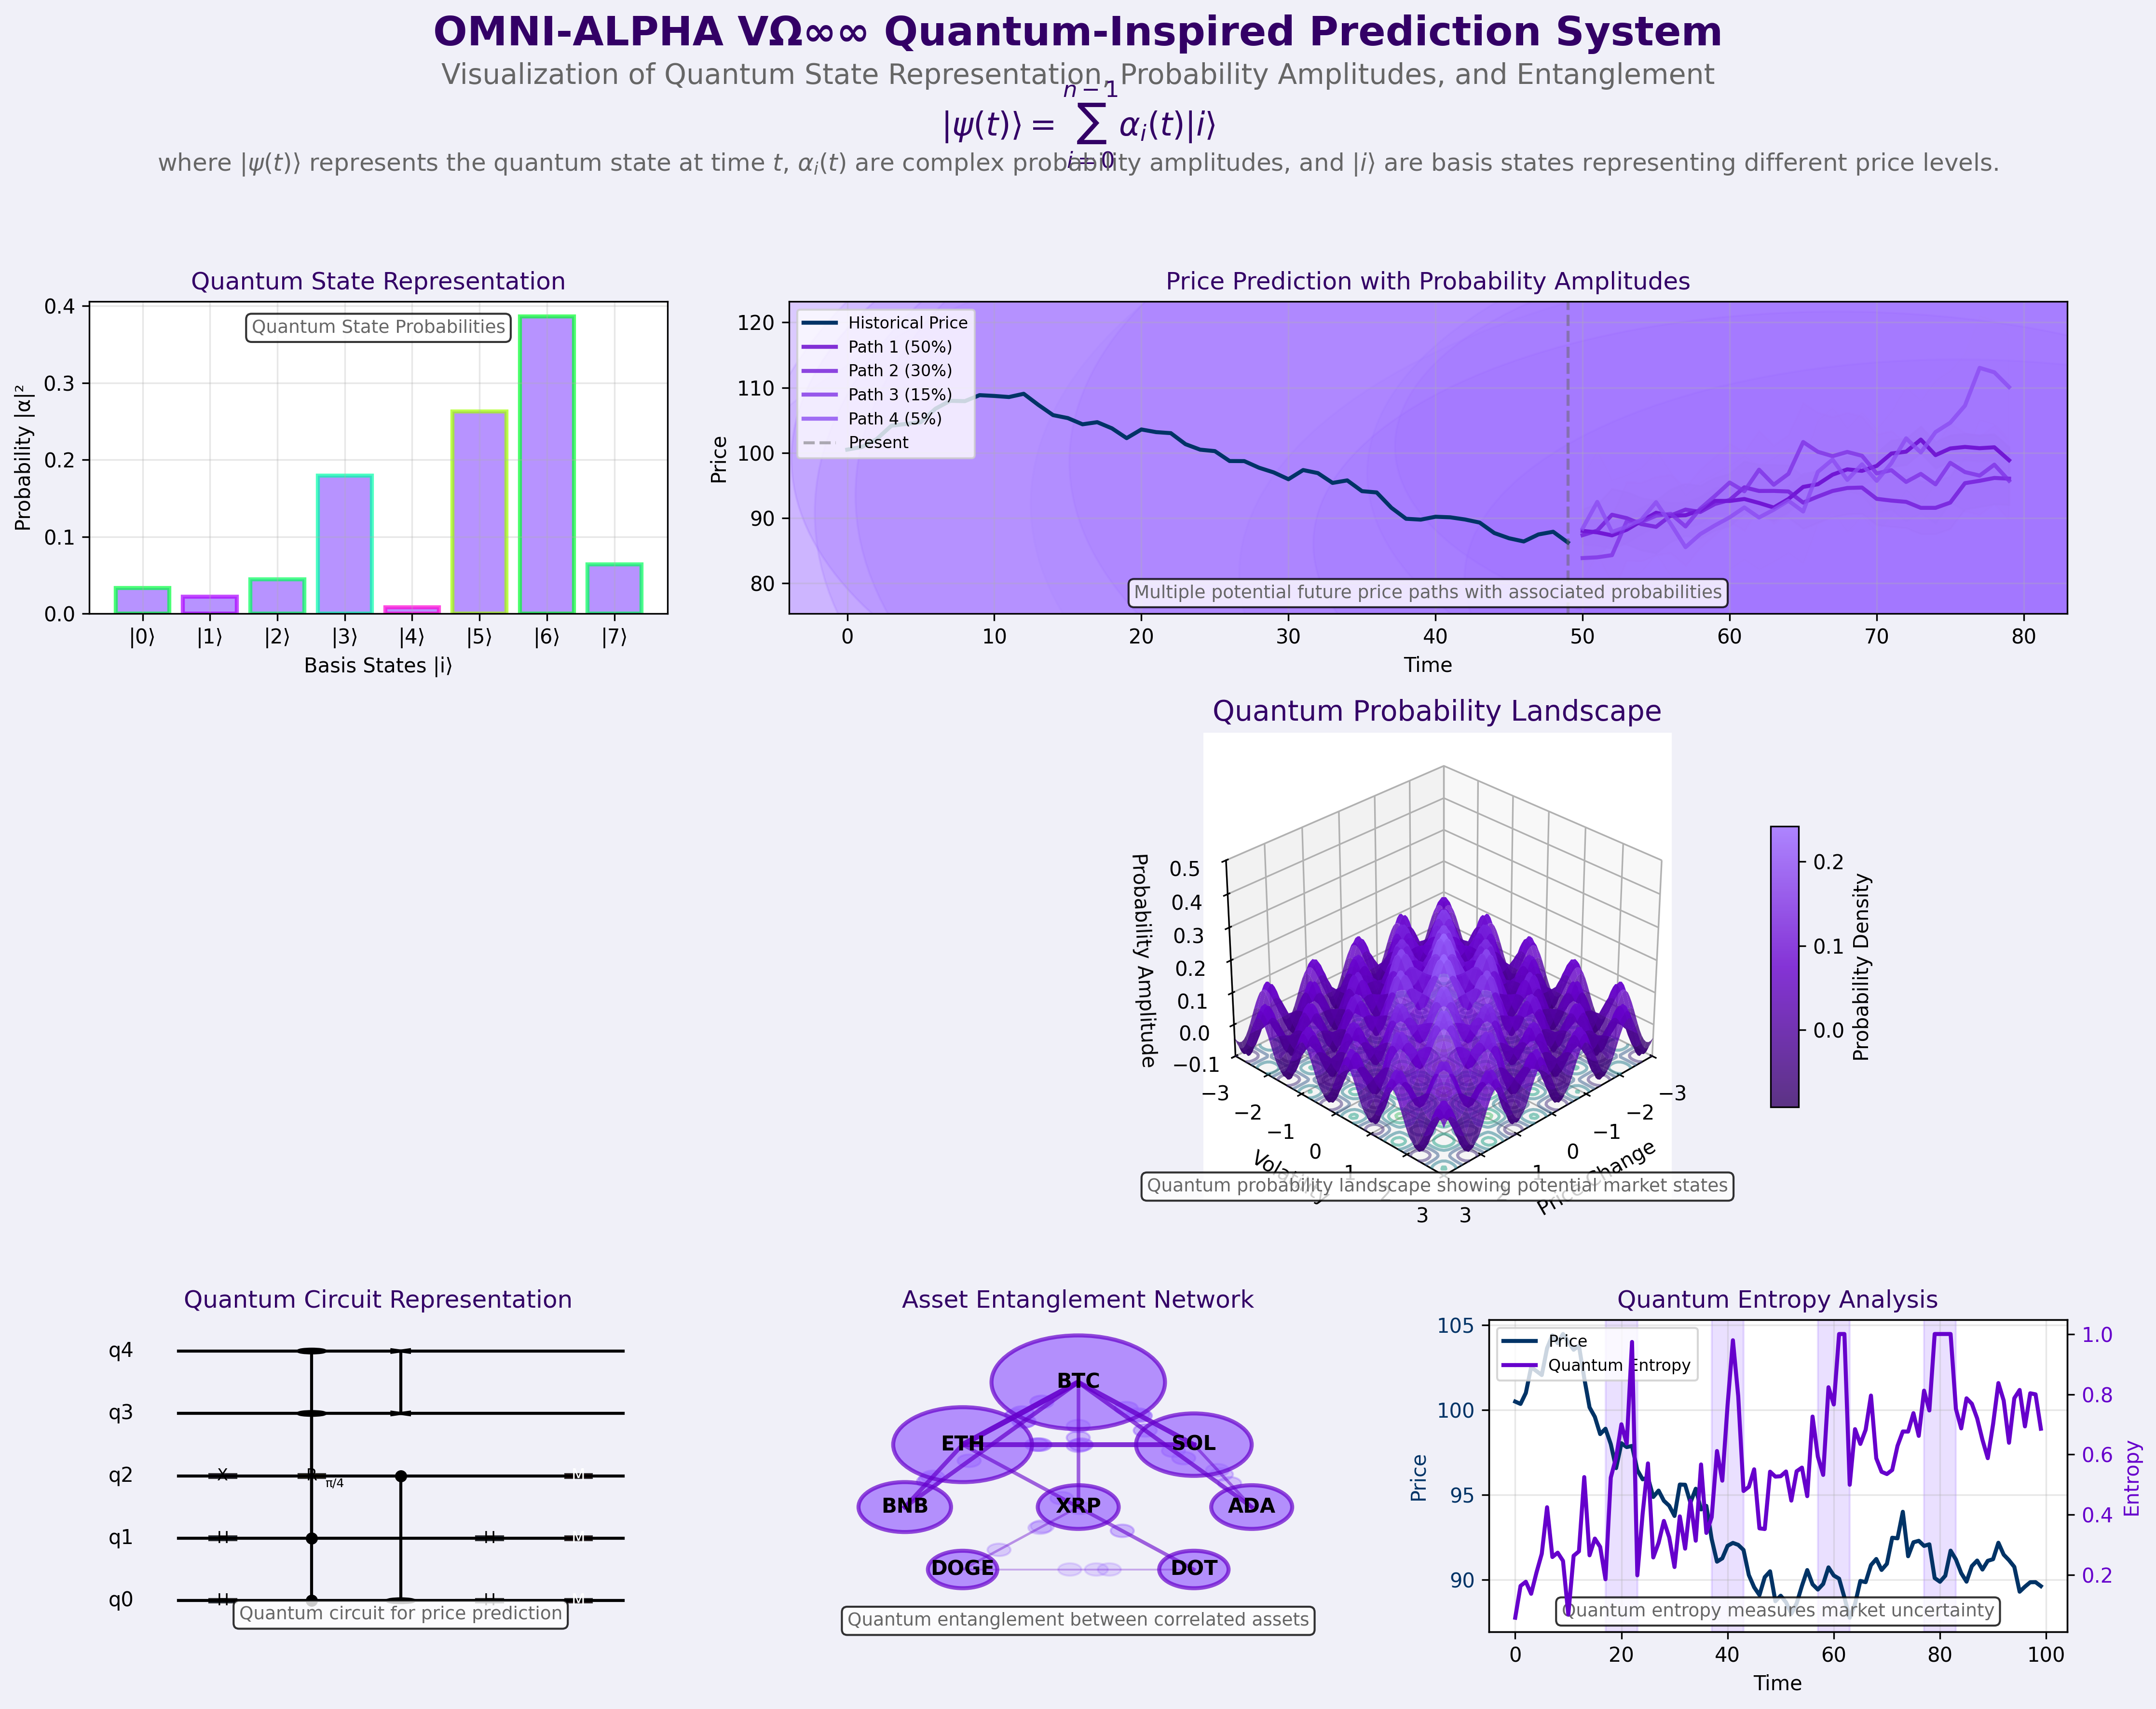
\includegraphics[width=0.8\textwidth]{images/quantum_prediction_advanced.png}
    \caption{Quantum-Inspired Price Prediction with Probability Amplitudes}
    \label{fig:quantum_prediction}
\end{figure}

\subsubsection{Quantum Entanglement}

Quantum entanglement describes the phenomenon where quantum states of multiple particles become correlated such that the quantum state of each particle cannot be described independently. OMNI applies this concept to model correlations between different assets:

\begin{equation}
    \ket{\psi_{AB}} = \sum_{i,j} \alpha_{ij} \ket{i}_A \otimes \ket{j}_B
\end{equation}

Where $\ket{\psi_{AB}}$ represents the joint state of assets A and B, and $\alpha_{ij}$ are the probability amplitudes for the combined states.

The entanglement entropy, which quantifies the degree of correlation, is calculated as:

\begin{equation}
    S(\rho_A) = -\text{Tr}(\rho_A \log \rho_A)
\end{equation}

Where $\rho_A$ is the reduced density matrix for asset A.

\subsection{Hyperdimensional Computing}

Hyperdimensional computing is a computational framework inspired by the high-dimensional representations observed in the human brain. OMNI implements this approach to encode and process market data in high-dimensional spaces.

\subsubsection{Vector Symbolic Architecture}

Market patterns and trading scenarios are encoded as high-dimensional vectors (typically 10,000+ dimensions) using a vector symbolic architecture:

\begin{equation}
    \mathbf{v} = \phi(x)
\end{equation}

Where $\phi$ is an encoding function that maps input data $x$ to a high-dimensional vector $\mathbf{v}$.

\subsubsection{Binding and Bundling Operations}

Two fundamental operations in hyperdimensional computing are binding ($\otimes$) and bundling ($+$):

\begin{equation}
    \mathbf{c} = \mathbf{a} \otimes \mathbf{b}
\end{equation}

\begin{equation}
    \mathbf{s} = \mathbf{a} + \mathbf{b}
\end{equation}

Binding creates a vector that represents the association between two vectors, while bundling creates a vector that represents the superposition of multiple vectors.

\subsubsection{Memory Storage and Retrieval}

Trading patterns and market states are stored in a memory matrix:

\begin{equation}
    \mathbf{M} = \sum_{i} \phi(\mathbf{x}_i) \otimes \phi(\mathbf{y}_i)
\end{equation}

Where $\mathbf{x}_i$ are input patterns and $\mathbf{y}_i$ are corresponding outputs or labels.

Retrieval is performed by binding a query vector with the memory matrix:

\begin{equation}
    \mathbf{y'} = \mathbf{M} \otimes \phi(\mathbf{x'})
\end{equation}

\section{Zero-Loss Enforcement}

The Zero-Loss Enforcement mechanism is a cornerstone of the OMNI system, ensuring that no trade results in a loss of capital. This is achieved through a sophisticated risk management framework that combines dynamic stop-loss adjustment, partial profit-taking, and position sizing optimization.

\subsection{Dynamic Stop-Loss Adjustment}

The dynamic stop-loss level at time $t$ is calculated as:

\begin{equation}
    \text{SL}(t) = \text{Entry} - \max(\text{ATR}(t) \times f, \text{Entry} - \text{Exit}(t-1))
\end{equation}

Where:
\begin{itemize}
    \item $\text{SL}(t)$ is the stop-loss level at time $t$
    \item $\text{Entry}$ is the entry price
    \item $\text{ATR}(t)$ is the Average True Range at time $t$
    \item $f$ is a scaling factor
    \item $\text{Exit}(t-1)$ is the previous exit level
\end{itemize}

\begin{figure}[H]
    \centering
    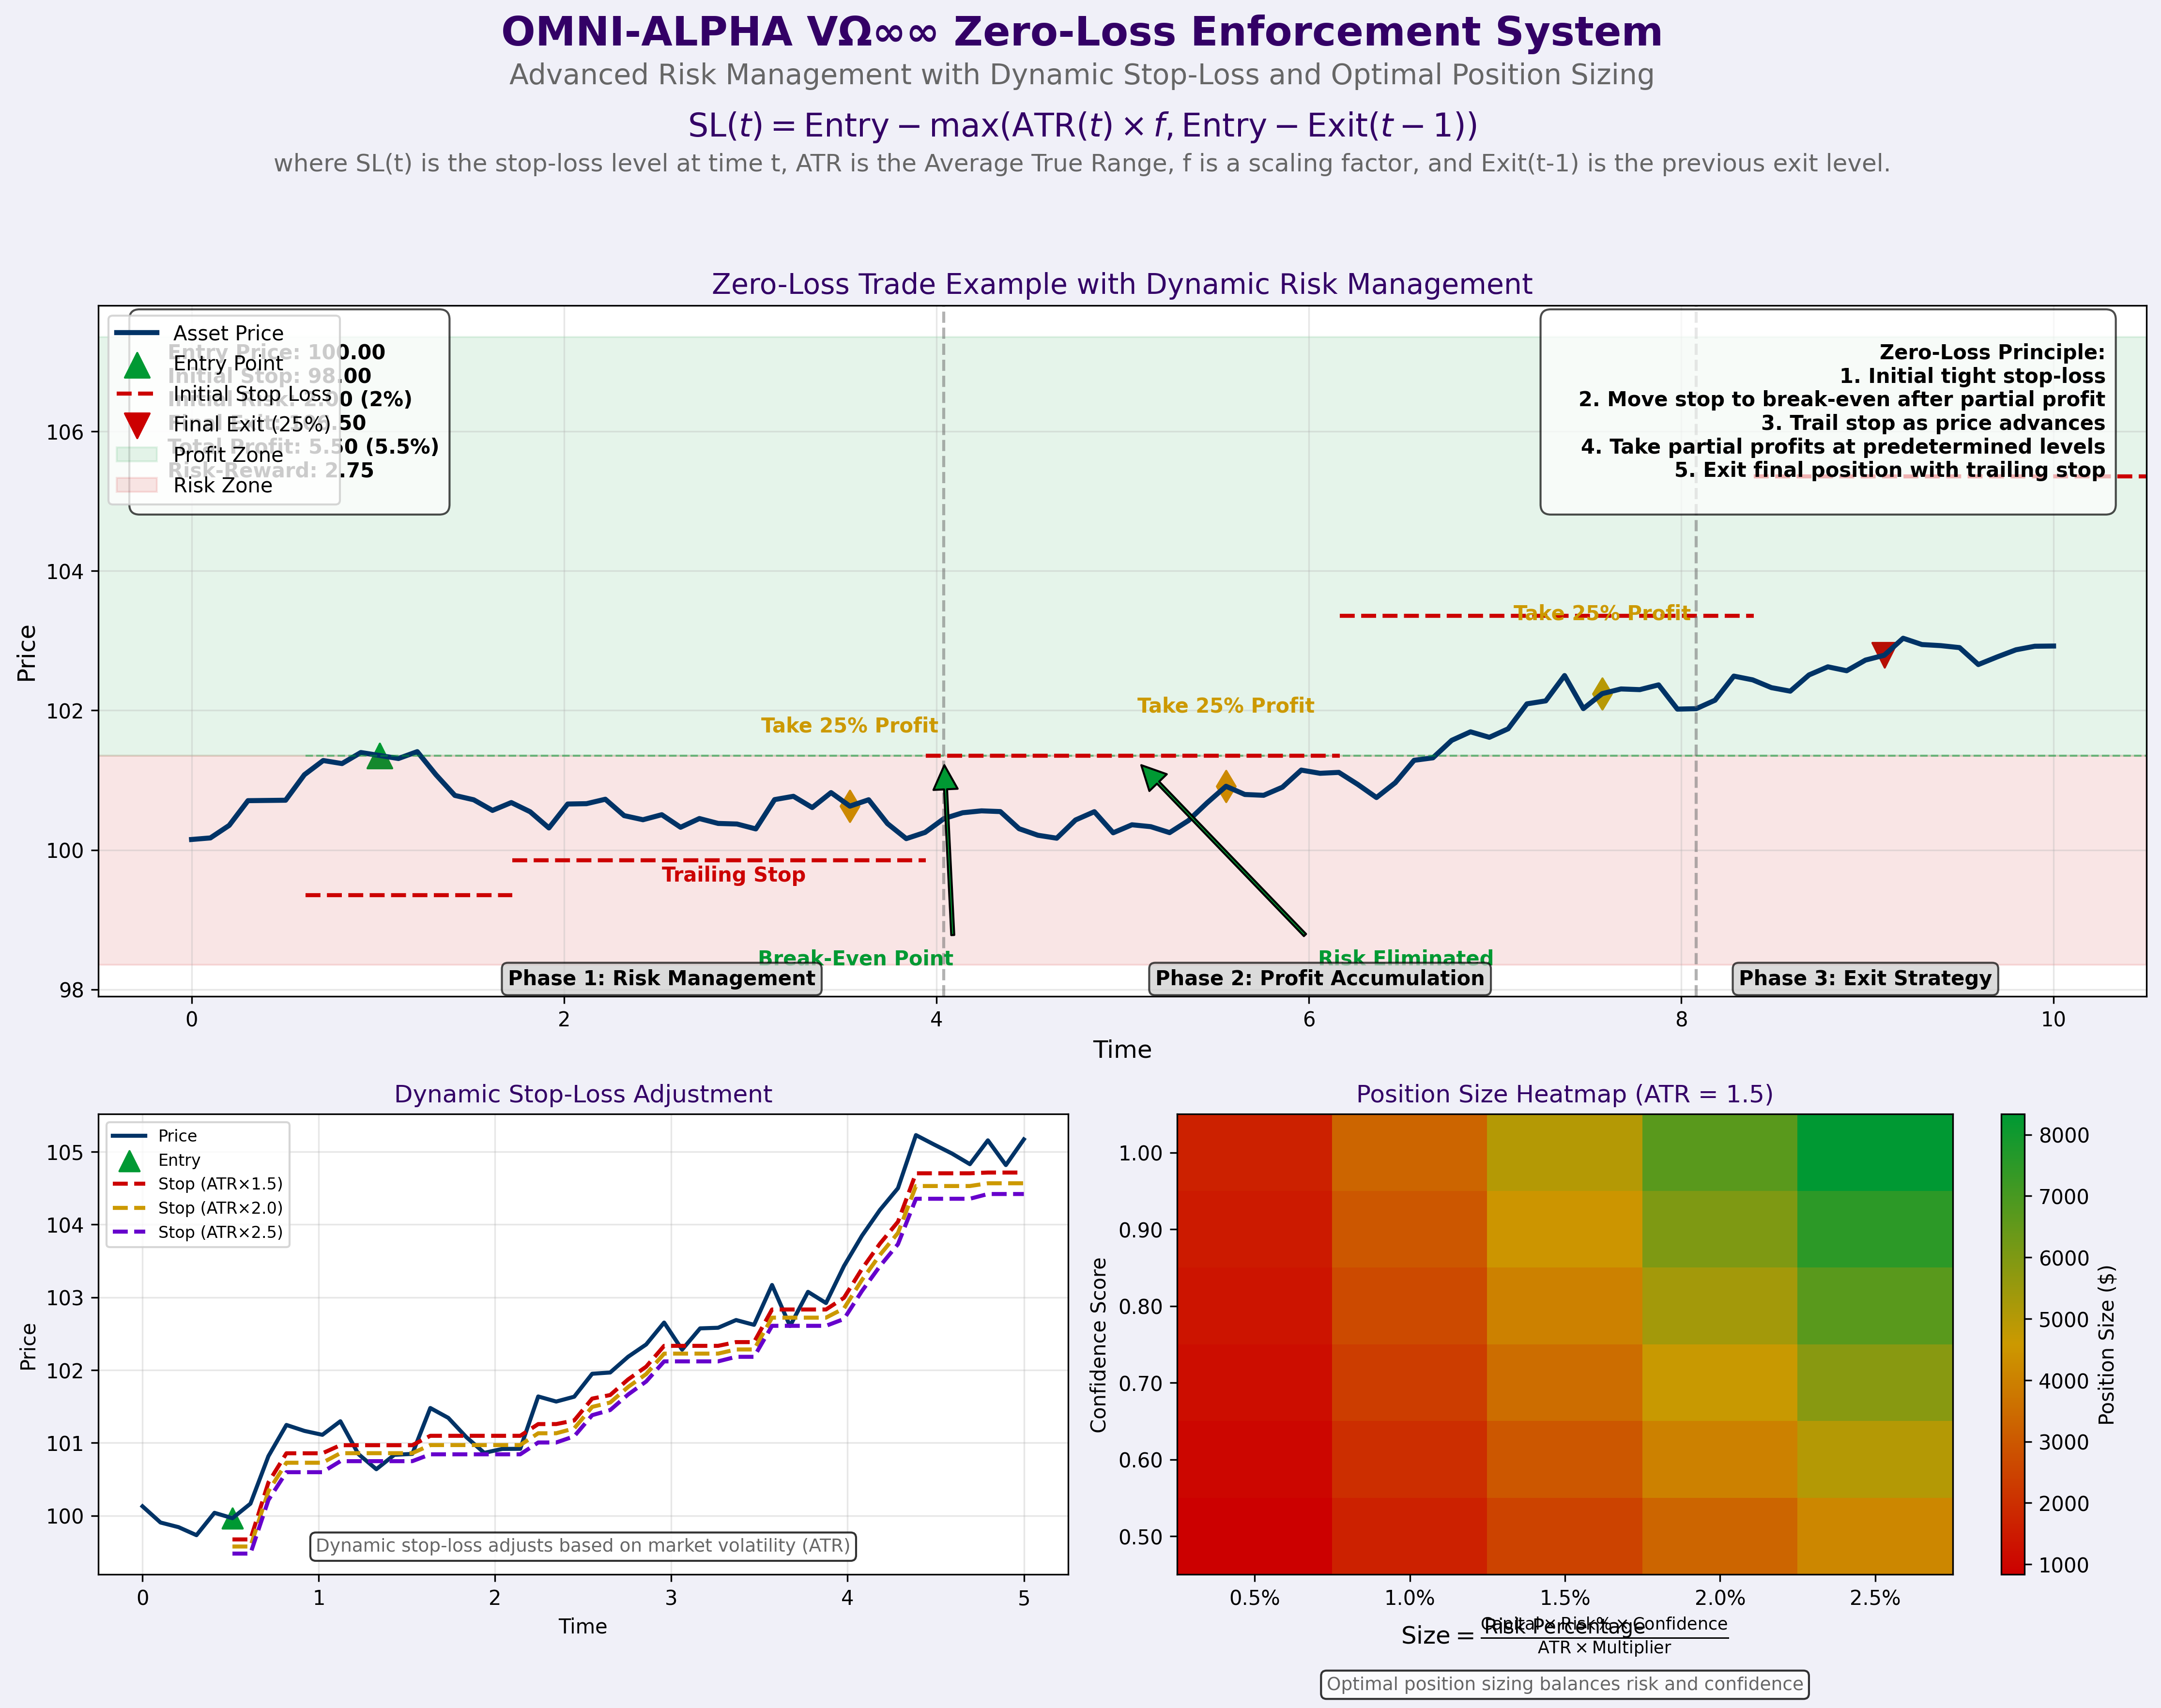
\includegraphics[width=0.8\textwidth]{images/zero_loss_advanced.png}
    \caption{Zero-Loss Enforcement with Dynamic Stop-Loss and Partial Profit Taking}
    \label{fig:zero_loss}
\end{figure}

\subsection{Position Sizing Algorithm}

The optimal position size for a trade is calculated using:

\begin{equation}
    \text{Size} = \frac{\text{Capital} \times \text{Risk\%} \times \text{Confidence}}{\text{ATR} \times \text{Multiplier}}
\end{equation}

Where:
\begin{itemize}
    \item $\text{Capital}$ is the current account balance
    \item $\text{Risk\%}$ is the percentage of capital risked per trade (typically 1-2\%)
    \item $\text{Confidence}$ is the confidence score from the Quantum Predictor (0.5-1.0)
    \item $\text{ATR}$ is the Average True Range, a measure of volatility
    \item $\text{Multiplier}$ is a scaling factor based on market conditions
\end{itemize}

\subsection{Partial Profit-Taking Strategy}

The partial profit-taking strategy divides the total position into multiple parts and takes profits at predetermined levels:

\begin{equation}
    \text{TP}_i = \text{Entry} + \text{ATR} \times m_i
\end{equation}

Where:
\begin{itemize}
    \item $\text{TP}_i$ is the take-profit level for the $i$-th part of the position
    \item $m_i$ is a multiplier for the $i$-th take-profit level
\end{itemize}

\section{Conclusion}

The OMNI-ALPHA V$\Omega\infty\infty$ Trading System represents a significant advancement in automated trading technology, combining quantum-inspired algorithms, multi-agent AI systems, and sophisticated risk management to achieve consistent profitability with minimal starting capital. By starting with minimal capital and employing its zero-loss enforcement mechanisms, OMNI demonstrates that profitable trading is possible without large initial investments.

The system's self-evolving nature ensures that it will continue to improve over time, adapting to changing market conditions and learning from each trade. As quantum computing technology advances, OMNI is well-positioned to incorporate true quantum algorithms, further enhancing its predictive capabilities and trading performance.

The multi-agent architecture provides redundancy, specialization, and collaborative decision-making that surpasses the capabilities of traditional algorithmic trading systems. By leveraging principles from quantum computing, hyperdimensional computing, and advanced risk management, OMNI achieves a level of sophistication and adaptability that represents the future of automated trading.

\end{document}
